\section{Results and Discussion} \label{results}



\subsection{Performance}\label{performance}
The temporal dynamics of a molecular system can be described by the \acrfull{cme}\cite{kampen_stochastic_2011}.
\acrfull{gssa}\cite{gillespie_general_1976} simulates these stochastic dynamics directly returning a set of individual trajectories for a list of particles observed.
In order to obtain accurate estimates of the average dynamic within a population of cell (\ie{} the mean dynamics), it is however necessary to perform multiple (often more than $10^4$) simulations.
Despite recent efforts \cite{niemi_efficient_2011,dittamo_optimized_2009,komarov_accelerating_2012} to provide fast implementation of this algorithm, computation remains extremely expensive. 
This time-complexity is a limiting factor in downstream analysis techniques, for
instance parameter inference that often requires repetition of these experiments for a large set of parameter values.

This particular limitation led to the development of approximations such as \acrfull{lna}\cite{komorowski_bayesian_2009} and \acrfull{mea}\cite{ale_general_2013}
 which model the mean behaviour directly, without evaluating the individual particle behaviours, and therefore can perform in a more realistic time.

Since the main driving force for development of these approximation algorithms is the potential reduction of the time taken to perform the analysis, 
it is paramount to make the implementation as efficient as possible.

In this section, we explore the implementation factors that influence the runtime of the algorithm, and describe the optimisations done to increase the its performance.
In particular, we show that symbolic computations can be limiting the algorithm and explain the techniques used to optimised them.
We also quantify the increase in performance we achieved and show that it is several orders of magnitude faster than the original \mat{} implementation.
In addition, we explore other limiting factors we have less control of, such as the choice of \gls{ode} solver, and discuss their potential implications to the analysis of biological systems.

\subsubsection{Optimising \acrlong{mea}}
\label{sec:optimising_mea}

\gls{mea} involves derivation of a system \gls{ode}s from a model.
This procedure\cite{ale_general_2013}, involves lengthy symbolic calculations.
Even for very simple models (\eg{} three species, five reactions), they cannot be realised manually.
The number equations in the generated \gls{ode} system, for a model with $s$ species and up to moments of order $o$ can be estimated by the following equation: 
\begin{equation}
    \text{Number of equations} = {{s + o} \choose {s}} - 1
    \label{eq:number_of_equations}
\end{equation}
As a consequence, the complexity of the calculation is predicted to increase exponentially with the number of species in the system and the maximal order of moments. 
For example, in a system with five species,  performing \gls{mea} up to moments of order 2, 3, 4 and 5, results in an \gls{ode} system with  20, 55, 125 and 251 equations, respectively. 

%In order to perform symbolic computations, we have used \sympy{} \cite{sympy_development_team_sympy:_2014}; a \py{} implementation of
%the symbolic computation routines.

In order to increase the scalability of the method, we have identified significant bottlenecks in our procedures using \py{} profiling tools.
We have then attempted to iteratively remove these bottlenecks one by one. Figure~\ref{fig:mea_speed} shows the cumulative effects of different optimisations.
The performance assessment were realised on algorithm when performing log-normal closure in order to show the effect of improvements specific to parametric closure (fig.~\ref{fig:mea_speed}d). 

\begin{figure}[tbh]

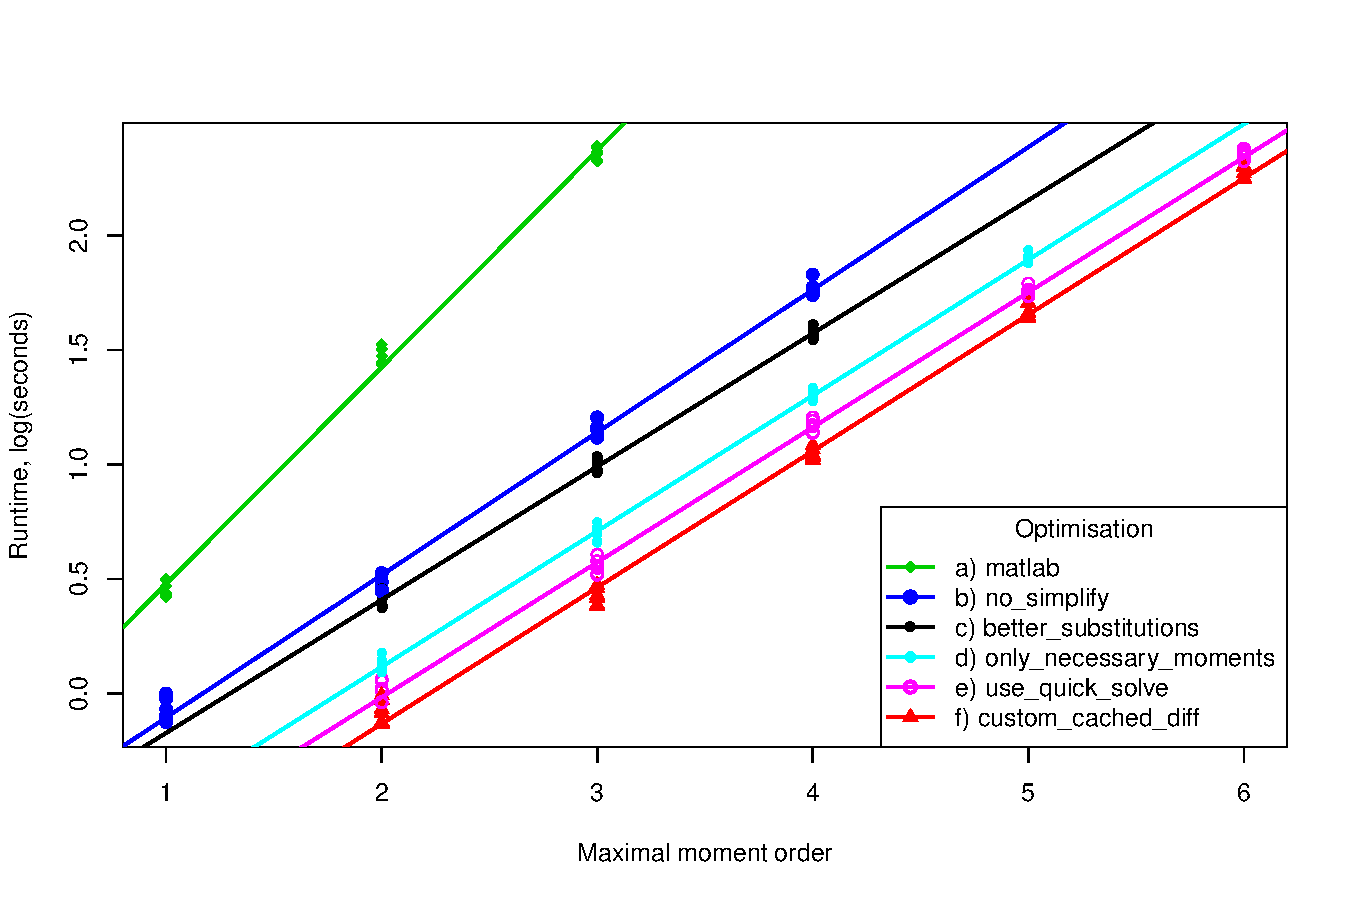
\includegraphics[width=0.95\textwidth{}]{../figure_mea_speed/mea_speed.pdf}
\caption{\emph{Cumulative performance improvement of symbolic 
calculations resulting from optimisation}.
The processing time for computing log-normal closure on \pft{} model with different maximal moment orders were measured for original Matlab implementation (a) and different optimisations (b$-$f).
In a first place, the calls to \texttt{sympy.simplify()} where removed (b). 
Then, \texttt{sympy.xreplace()} was used instead of \texttt{sympy.substitute()} (c). 
Generating an $(n-s) \times (n_2-s + 1)$ matrix (d), as opposed to an $(n-s) \times (n-s + 1)$ one, also increase speed.
Implementing a simplified equation solver instead of using \texttt{sympy.solve()} also resulted in a significant speed-up (e). 
Finally, caching (memorisation) \texttt{sympy.diff()} allowed even better performance.
The time complexity appears exponential ($O(2^n)$, where $n$ is the maximal moments order) in every case, 
%Interestingly, the slopes between, a ($0.95$) and c ($0.58$), and b ($0.62$) and c were significantly different ($p-value <10^{-15}$ and $p-value = 3 \times 10^{-4}$, respectively; t-test on the slopes of the linear regression). 
%No significant difference was found between the slopes of the subsequent optimisations (c$-$f). 
%However, the intercepts were significantly smaller between each consecutive optimisations after c) ($p-value < 10^{-6}$ for all; t-test on the intercepts of the linear regression).
Nine replicates were performed on the same CPU. 
For optimisation c$-$f, values corresponding to maximal order moments lower than two were removed because of the inherent inaccuracy in measuring very short durations
}
\label{fig:mea_speed}
\end{figure}

\quentintodo{move the stats here}

Reorganising, profiling and rewriting the code resulted in incremental significant performance improvements of symbolic computations in \means{} compared to the original \mat{} code.
For instance, with the same \pft{} system and closure method, 
we predict that computation up to \gls{ode}s up $8^{th}$ order will take 46 minutes with \means{}, 5 hours after the first optimisation (fig.~\ref{fig:mea_speed}b) and as much as 148 days with the original implementation.
These improvement have allowed us to explore the performance of MEA in higher depth, and will hopefully contribute to make \gls{mea} realistically usable for systems with more species and reactions.

\subsubsection{Evaluating Expressions Efficiently}

\sauliustodo[inline]{QG: reviewed, what do you think ?}

As mentioned in the introduction to this section, the reduction of computational cost was the main reason for developing of approximation methods.
As described in the previous section, in order to be able to explore the approximation methods in more depth,
we needed to make the generation of the set of equations as efficient as possible. 

Generating a set of equations (\ie{} and \gls{ode} problem) is generally only the first step.
In most cases, the result is used to perform simulations with different parameters.
As a consequence, the same \gls{ode} problem will be generated once, and used many times.
Typically, a user would spend some time to generate an set of equation using \gls{mea}, and then use this \gls{ode} problem to perform hundreds of simulations.
Therefore, it was extremely important to assess and try to improve numerical evaluation performance.
 
%Even though it is a great improvement from the original prototype, 46 minutes is still a long time to wait for the computer to do the number crunching. 
%We can accept to wait this long, however, as we only need to do that once for a set of equations -- the next time we intend to do that, we can just read the previous set from a file.

%Evaluating these expressions is a completely different story however.
%Since we need to evaluate each expression hundreds, if not thousands of times when performing the simulations of the system,
% we want to make these tasks as efficient as possible, as every microsecond counts. 

In order to minimise the overhead of computations, we use the {\tt autowrap} module, built into {\tt sympy} to compile our numeric expressions into \texttt{C}
and then wrap the same \py{} interface around them so the end user does not see any difference.
This process bears some overhead, of course, as the system needs to be compiled for every simulation.

We notice that the expressions for a given set of equation could be compiled once and reused for all subsequent simulations on this set of equations.
Therefore, we used caching to keep precompiled expressions in memory.
 
As a consequence, the overhead is present only in the first evaluation of expressions, whilst all other evaluations are an order of magnitude faster.
This performance improvement is illustrated in the tutorial \autoref{sec:reuse_of_simulation_objects}.

\subsubsection{Comparing the Performance of Different \gls{ode} Solvers}

\sauliustodo[inline]{QG: reviewed, what do you think ?}
The symbolic expression evaluation speed, whilst incredibly important, contributes only partially to the scalability of the simulation procedures.
The performance of numerical \gls{ode} solvers themselves also plays a critical role.

These solvers differ in many ways ranging from a set of parameters to different heuristics and even algorithms.
Choice of the \emph{best} solver for an \acrlongpl{ode} system depends very much on the particular problem to simulate.
However certain solvers tend to be more generally adopted than others\cite{andersson_workbench_2012}.

CVODE\cite{hindmarsh_sundials_2005} is an example of one of the most widely used solvers.
As described in \autoref{sec:ode_simulations}, we implement two variants of this solver, \verb#ode15s# and \verb#cvode#.
Both solvers point to the same back-end implementation of CVODE provided by \verb#assimulo# package\cite{andersson_christian_assimulo:_????}.
The only diference is that \verb#ode15s# solver's default parameters mimics the eponymous \mat{} solver.

Besides CVODE solvers, our package is able to perform simulations with seven other solvers, using completely different algorithms.
The complete list of available solvers used in available in the documentation\citationneeded{refer to docs}.
Naturally, it was interesting to compare the respective performance of different solvers on our type of problems.

In order to measure the runtime performance of the solvers, we performed a set of simulations of the \acrlong{mea} of the \pft{} model.
We deliberately chose two sets of parameters: one that we know is fairly stable and easy to simulate with, so called \emph{safe} parameter set,
and another parameter set that is known to cause the trajectories to become stiff and therefore cause problems to the solvers.
We call the latter parameter set the \emph{unsafe}.
 
\begin{figure}[tb]
   \centering
   \begin{subfigure}[t]{0.45\textwidth}
       \includegraphics[width=\textwidth]{../pipeline/task-output/solver-runtimes/runtimes-ode15s.pdf}
       \caption{\texttt{ode15s}}
       \label{fig:runtimes-safe-unsafe-ode15s}
   \end{subfigure}
   ~
   \begin{subfigure}[t]{0.45\textwidth}
       \includegraphics[width=\textwidth]{../pipeline/task-output/solver-runtimes/runtimes-euler.pdf}
       \caption{Euler}
       \label{fig:runtimes-safe-unsafe-euler}
   \end{subfigure}
   
    \caption{Comparison of the time taken for the {\tt ode15s} and Euler solvers to simulate a system, with respect to two parameter sets, one harder to simulate than the other as it makes the problem stiff.
    The time axis is in log-scale. Regression lines through the marked points is represented.
    Note that the number of equations increases exponentially with maximum order, essentially making this a log-log plot.}
\label{fig:runtimes-safe-unsafe}
\end{figure}

\texttt{ode15s} solver was more performant for the safe parameter set (fig.~\ref{fig:runtimes-safe-unsafe-ode15s}).
Heuristic solvers tend to automatically adjust the step size depending on the problem in hand, adjusting for the rate of stochastic events being simulated.
It is therefore expected that they would perform worse for stiff problems, where the timeframes between the events become shorter and shorter, which requires more time steps.

In contrast, Euler solver, uses a constant step size, and therefore the runtimes for the two parameter sets are equal (\autoref{fig:runtimes-safe-unsafe-euler}).

Since \gls{ode} solvers are inherently heuristic, their CPU performance may suffer considerably for unstable systems.

We were then interested in assessing, in the same fashion, all nine available solvers for these two parameter sets (\autoref{fig:solver-runtimes}).
\sauliustodo[inline]{Describe these results, after you get some sleep}

\begin{figure}[bt]
    \centering
    \includegraphics[width=\textwidth]{../pipeline/task-output/solver-runtimes/runtimes-all.pdf}
    \caption{Comparison of all solver runtimes}
    \label{fig:solver-runtimes}
\end{figure}

In order to improve performance, we have compared solvers on the basis of their speed.
However, they also differ in their accuracy and stability.
This was investigated in  \sauliustodo{ref to new section once I create it}.

\subsection{Moment Expansion Closure}

In \gls{mea} the time derivative of each central moment is expressed in terms of the higher order moment. 
This behaviour essentially has no upper bound and continues to the moments of infinite order. 
Since we cannot evaluate these expressions in the limit analytically, it is necessary to ``close'' the expansion by providing a closed form for the higher order moments.
This also makes the method an ``approximation" rather than an exact method.

In the original work \cite{ale_general_2013}, higher order central moments are assumed to be equal to zero.
This is very convenient, but is a strong and not necessarily valid assumption. 

As an alternative, parametric probability distribution can be used to express moments of arbitrary orders. 
For instance, a multivariate normal distribution is parametrised only by means (\ie{} first order raw moment)
and a covariance matrix (\ie{} second order central moments). 
As a consequence, it is possible to express any arbitrary moment from means, variances and covariances. 
A promising area of research involves closing moment expression by parametric forms of highest order central moments instead
of assuming them to be null.
Preliminary work \cite{lakatos_preparation_2014} suggests that using a parametric distributions for \gls{mea} is, in some cases, a better approximation.
In addition, Ale \emph{et al.} predicted that ``including more moments would improve the estimation''\cite{ale_general_2013}.

The dramatic improvement in performance compared to the \mat{} prototype (see \autoref{sec:optimising_mea}) has rendered the exploration of higher-order and parametric moment closures possible.
Therefore, we were naturaly interested in investigating the effect of maximal moment order and different type of closures on the quality of the approximation.
igure~\ref{fig:max_order_and_closure_on_distance_summary} summarises our resutlts on the \pft{} model.

\begin{figure}[t]
    \centering
    \includegraphics[width=0.95\textwidth]{../pipeline/task-output/FigureP53Summary/FigureP53Summary-pdf-7.pdf}
    \caption{\emph{Effect of different closure methods and maximal moment order on simulation accuracy}. The \pft system was modelled using \gls{mea} with five types of closure and for maximal moment order up to seven.
Resulting trajectories were all compared to an average of 5000 \gls{gssa} simulations using sum of square distance (a).
Distance is in log scale. Missing values indicate solver failure for that particular set of parameters.}
    \label{fig:max_order_and_closure_on_distance_summary}
\end{figure}

The \pft{} system, with parameters from \cite{ale_general_2013}, was investigated.
As mentioned earlier it is expected that the approximation accuracy increases with the maximal moment order, \ie{} distance to \gls{gssa} obtained should decreases
 as maximal moment order increases. 
For normal and scalar closures, this trend we observe this trend up to maximal moment order six. 
However, this does not stand for seventh order moment.

\quentintodo[inline]{Todo double check the labels in the legend, was it really normal that was worse and scalar that failed?}

As seen in the figure, the closure using the normal distribution had performed worse than the sixth order closure when maximum order was set to seven.
We could not obtain the result for the seventh order closure using the standard scalar closure, as the ODE solver has failed simulating the problem, which usually indicates a ``stiff'' \gls{ode} problem\citationneeded{stiff odes}. 
The generated trajectories are shown in \autoref{fig:max_order_and_closure_on_distance_trajectories}. 
Trajectory generated from the normal distribution closure seem to `mismatch' the trajectory obtained from the \gls{gssa} simulations by a margin.
% (\emph{purple line, subplot on the right-hand-side}). 

The reason for this behaviour is uncertain; it might be a limitation of the approximation method, or a numerical limitation of the available \gls{ode} solver.
It is hard to know which explanation is more likely since we cannot test the two hypotheses separately. 
Interestingly, we observed a similar behaviour with all of the solvers tested, which is further explored in \sauliustodo{link to my section where we study the phenomenon on larger scale with different solvers}.

Note that for even maximal moment orders, normal and scalar are identical.
When the maximal moment order is even, it means that the perametric expression of an odd (the next) order moment was used for closure.
Normal distribution is symmetrical. One consequence is that odd central moments are always zero. 
For instance, the sckew (\ie{} third order central moment) of a normal distribution is zero.
Therefore, this behaviour is perfecty normal.


\begin{figure}
    \centering
    \includegraphics[width=0.95\textwidth]{../pipeline/task-output/FigureP53Simple/FigureP53Simple-pdf-7.pdf}
%~
    \caption{\emph{Complete trajectories of a single species (\pft) for max order three and seven are shown} Black lines indicate the average of \gls{gssa} simulations. Missing lines, compared to the legend in  m\autoref{fig:max_order_and_closure_on_distance_summary} indicate solver failure.}
    \label{fig:max_order_and_closure_on_distance_trajectories}
\end{figure}

 
for log-normal closure, the ground truth trajectory seems to be well approximated when the maximal moment order is three, but the approximation gets less and less accurate for higher maximal order moments.
A deeper look at the trajectories indicate that, in this latter case,
oscillations are damped too quickly, as opposed to the behaviour seen using normal closure, where the oscillation amplitude increases (see \autoref{fig:max_order_and_closure_on_distance_trajectories}, red line).

Interestingly, for even maximum moment order (\ie{} 2, 4, 6) log-normal closures generated \gls{ode}s which, despite our efforts, could not be numerically solved.

Finally, it seems that the results obtained from multivariate distribution closures and  univariate distribution closures, which do not model the covariance terms, are the same for this particular system. 
This is not true for all of the systems. 
For instance, we have observed that in the \emph{hes1}, it is advantageous to model covariance (data not show).
\quentintodo{put hes1 exple if time}

Surprisingly, higher order moment closure did not necessarily result in better approximations.
In addition, our results indicate that there might be a complex interaction between the type of closure and the maximal moment order. 
Unfortunately, this makes it difficult to define \emph{a priori} which closure and maximal moment order should be used for a given system.
These unexpected results lead us explores this phenomenon on wider scale of parameters\sauliustodo{link to the section}.

\subsection{Parameter Inference using \acrlong{mea}}
Parameter inference procedure aims to obtain the correct parameter values for the system by exploring the parameter space and comparing the simulation trajectories with the experimental data.

%In order to study the performance of the parameter inference procedure using \acrlong{mea}, we took the average trajectory obtained from the  $5000$ \gls{gssa} simulations of the \pft{} with a certain parameter set and used it as the observed dataset we want to infer the parameters from. Essentially, the inference procedure is expected to return the said parameter set back to us.
In order to study the performance of the parameter inference procedure using \acrlong{mea},
we generated $5000$ \gls{gssa} simulations of the \pft{} with a certain parameter set.
Then, we used the average as an observed dataset from which to infer parameters.
In this way, we know exactly what are the ``true'' parameters.

In order to determine the base case performance, we performed the parameter inference using the \pft{} model expressed only in terms of the first order moments (see \autoref{fig:7_dimensional_parameter_space}).
This approximation is bound to be very inaccurate for the particular system, as higher order moments are necessary to capture the damped oscillations present in the means of \gls{gssa} simulations\cite{ale_general_2013}.


\begin{figure}
\centering
\includegraphics[width=0.9\textwidth]{{../pipeline/task-output/SevenDimensionalInferenceFigure/SevenDimensionalInferenceFigure-pdf-ode15s--sum_of_squares-5000}.pdf}
\caption{\emph{Distance landscape based on inference using all the parameters in \pft{} model.}
In the parameter inference procedure, all seven parameters were free and started from the correct values.
The parameters are aligned both horizontally and vertically to display the distance landscape obtained by comparing inferred trajectories with \gls{gssa} trajectories.}
\label{fig:7_dimensional_parameter_space}
\end{figure}


The starting parameters were the correct ones, so we expected immediate convergence (\ie{} no movement in the parameter space).
Surprisingly, when parameters are free, inference was able to find a different set of parameters for which observed and theoretical trajectories are extremely similar.
This result was unexpected, because, in this case, \gls{mea} was modelling means (no higher order moments).

The set of parameters obtained by inference were very different from the ``true'' parameters (from \gls{gssa} simulations),
but the approximated trajectories were identical (see \autoref{fig:parameter_pairs}).
This strongly questions the suitability of parameter inference procedures in obtaining the correct parameter sets.

\begin{figure}
    \centering
    \begin{subfigure}[t]{0.9\textwidth}
    \includegraphics[width=\textwidth, height=0.18\textheight]{{../pipeline/task-output/FigureInferenceStartEndSSA/Paired-parameters-c2-c6}.pdf}
    \label{fig:parameter_pair_c2_c6}
    \caption{Parameter pair $c_2$ and $c_6$}
    \end{subfigure}
    ~
    \begin{subfigure}[t]{0.9\textwidth}
    \includegraphics[width=\textwidth, height=0.18\textheight]{{../pipeline/task-output/FigureInferenceStartEndSSA/Paired-parameters-c0-c1}.pdf}
    \label{fig:parameter_pair_c0_c1}
    \caption{Parameter pair $c_0$ and $c_1$}
    \end{subfigure}
    ~
    \begin{subfigure}[t]{0.9\textwidth}
    \includegraphics[width=\textwidth, height=0.18\textheight]{{../pipeline/task-output/FigureInferenceStartEndSSA/Paired-parameters-c0-c6}.pdf}
    \label{fig:parameter_pair_c0_c6}
    \caption{Parameter pair $c_0$ and $c_6$}
    \end{subfigure}
    ~
    \begin{subfigure}[t]{0.9\textwidth}
    \includegraphics[width=\textwidth, height=0.18\textheight]{{../pipeline/task-output/FigureInferenceStartEndSSA/Paired-parameters-c1-c6}.pdf}
    \label{fig:parameter_pair_c1_c6}
    \caption{Parameter pair $c_1$ and $c_6$}
    \end{subfigure}
    ~
    \caption{\emph{Four parameter pairs can produce a perfect match between inferred optimal trajectories and SSA trajectories for all species in \pft{} model.}
    The distance from the SSA trajectory for each species is displayed in each subfigure.
    Trajectories are simulated using maximum order 1. The three columns in each row represent the three species in the \pft{} model.}
    \label{fig:parameter_pairs}
\end{figure}

%\sisitodo[inline]{Why don't we compare the SSA trajectories with these parameters somewhere as well, if there is time?}

In order to gain some insight into these unexpected inference results, we first attempted to restrict ourselves to, easier to comprehend, two-dimensional space.
To do this, we restricted our parameter inference procedure to only have only a pair of free parameters at a time (all other parameters are fixed to their true values).
We performed this for all combinations of two parameters and checked if we can reproduce the curious behaviour.

Interestingly, we were able to observe the same behaviour for the parameter pairs $c_2$ and $c_6$, $c_0$ and $c_1$, $c_1$ and $c_6$, and finally $c_0$ and $c_6$ (see \autoref{fig:parameter_pairs}).
We then have chosen the pair of parameters that allowed the inference procedure to converge to a trajectory with minimal distance to the stochastic average -- $c_2$ and $c_6$ for further investigations.


\begin{figure}
\centering
    \begin{subfigure}[t]{0.2\textwidth}
    \includegraphics[width=\textwidth]{{../pipeline/task-output/SampleMultidimensionInferenceFigure/SampleMultidimensionInferenceFigure-pdf-1-scalar-True-90.0_0.002_1.704_1.1_0.93_0.96_0.7822-ode15s--90.0_0.002_1.704_1.1_0.93_0.96_0.7822-sum_of_squares-5000}.pdf}
    \end{subfigure}
    ~
    \begin{subfigure}[b]{0.6\textwidth}
    \includegraphics[width=\textwidth]{{../pipeline/task-output/FigureInferenceStartEndSSA/FigureInferenceStartEndSSA-1-scalar-c2-1.7040-c6-0.7822}.pdf}
    \end{subfigure}
    ~
    \begin{subfigure}[t]{0.2\textwidth}
    \includegraphics[width=\textwidth]{{../pipeline/task-output/SampleMultidimensionInferenceFigure/SampleMultidimensionInferenceFigure-pdf-2-scalar-True-90.0_0.002_1.704_1.1_0.93_0.96_0.7822-ode15s--90.0_0.002_1.704_1.1_0.93_0.96_0.7822-sum_of_squares-5000}.pdf}
    \end{subfigure}
    ~
    \begin{subfigure}[b]{0.6\textwidth}
    \includegraphics[width=\textwidth]{{../pipeline/task-output/FigureInferenceStartEndSSA/FigureInferenceStartEndSSA-2-scalar-c2-1.7040-c6-0.7822}.pdf}
    \end{subfigure}   
    ~
    \begin{subfigure}[b]{0.2\textwidth}
    \includegraphics[width=\textwidth]{{../pipeline/task-output/SampleMultidimensionInferenceFigure/SampleMultidimensionInferenceFigure-pdf-3-scalar-True-90.0_0.002_1.704_1.1_0.93_0.96_0.7822-ode15s--90.0_0.002_1.704_1.1_0.93_0.96_0.7822-sum_of_squares-5000}.pdf}
    \end{subfigure}
    ~
    \begin{subfigure}[b]{0.6\textwidth}
    \includegraphics[width=\textwidth]{{../pipeline/task-output/FigureInferenceStartEndSSA/FigureInferenceStartEndSSA-3-scalar-c2-1.7040-c6-0.7822}.pdf}
    \end{subfigure}   
     ~  
    \begin{subfigure}[b]{0.2\textwidth}
    \includegraphics[width=\textwidth]{{../pipeline/task-output/SampleMultidimensionInferenceFigure/SampleMultidimensionInferenceFigure-pdf-4-scalar-True-90.0_0.002_1.704_1.1_0.93_0.96_0.7822-ode15s--90.0_0.002_1.704_1.1_0.93_0.96_0.7822-sum_of_squares-5000}.pdf}
    \end{subfigure}
    ~
    \begin{subfigure}[b]{0.6\textwidth}
    \includegraphics[width=\textwidth]{{../pipeline/task-output/FigureInferenceStartEndSSA/FigureInferenceStartEndSSA-4-scalar-c2-1.7040-c6-0.7822}.pdf}
    \end{subfigure}   
   
    \begin{subfigure}[b]{0.2\textwidth}
    \includegraphics[width=\textwidth]{{../pipeline/task-output/SampleMultidimensionInferenceFigure/SampleMultidimensionInferenceFigure-pdf-5-scalar-True-90.0_0.002_1.704_1.1_0.93_0.96_0.7822-ode15s--90.0_0.002_1.704_1.1_0.93_0.96_0.7822-sum_of_squares-5000}.pdf}
    \end{subfigure}
    ~
    \begin{subfigure}[b]{0.6\textwidth}
    \includegraphics[width=\textwidth]{{../pipeline/task-output/FigureInferenceStartEndSSA/FigureInferenceStartEndSSA-5-scalar-c2-1.7040-c6-0.7822}.pdf}
    \end{subfigure}
   
\caption{\emph{Distance landscape and trajectories at different maximal orders for \pft{} model.}  Among seven parameters, only the values for $c_2$ and $c_6$ are inferred, with starting values inferred from inference using the true values.
The left column displays distance landscapes, the warmer the colour, the more distant the inferred trajectories are from the \gls{gssa} trajectories.
The numbers in the distance landscape indicate the distance between optimal trajectories obtained from inference and the \gls{gssa} trajectories.
The \gls{gssa} trajectories are generated using the new parameter values labelled as \emph{start}.
Three trajectories are shown for each species.
The starting trajectories are simulated using the starting values are indicated above the trajectories, with $c_2$ and $c_6$ inferred using \emph{sum of squares} distance method.
Both the optimal and the \gls{gssa} trajectories are generated based on the end point in correspondent distance landscape.
The distance displayed for each species represent the distance between the optimal and \gls{gssa} trajectories.}
\label{fig:parameter_inference_landscape_trajectories}
\end{figure}




As seen in \autoref{fig:parameter_inference_landscape_trajectories}, the optimal trajectories obtained using inference are mostly overlaping with the \gls{gssa} trajectories,
especially for lower orders.
This result is suspicious, because the parameter values inferred, as indicated in the correspondent distance, is far from the true values\sisitodo{QG: I do not get this}.
In fact, the inferred value for $c_6$ can be more than 10 times larger than the true value, which is not meaningful biologically.
Furthermore, when using higher maximal order for inference, a slight gap between the optimal and \gls{gssa} trajectories does not imply better inference result,
because the inferred parameter values are still incorrect.

The deviation between inferred and correct parameter values can be explained using the distance landscape,
as the starting point \ie{} the true parameter values, can be distant from the minima.
As the maximal order increases, the distance gradient becomes less sharp, preventing the system from finding the minima.

In conclusion, these result raises interrogations about the validity of parameter inference approaches using \gls{mea} approximation.
